% Report on the 3x+1 Problem for Research Methods in Applied Maths
% 03.03.2020, Moritz Konarski, AUCA

\documentclass[12pt,a4paper,reqno]{amsart}
% packages used
\usepackage[english]{babel}
\usepackage[utf8]{inputenc}
\usepackage[T1]{fontenc}
\usepackage{amsmath}
\usepackage{amsfonts}
\usepackage{anysize}
\usepackage{textcomp}
\usepackage{graphicx}
\graphicspath{{../graphics/}}
\usepackage{epstopdf}
\usepackage[utf8]{inputenc}
\usepackage{fancyhdr}
\usepackage{lastpage}
\usepackage[hidelinks]{hyperref}
\hypersetup{
    colorlinks=true,
    linktoc=all,
    allcolors=black,
    final
}
% this command was found at:
% https://tex.stackexchange.com/questions/51851/change-distance-between-page-number-and-bottom-edge-of-page
\usepackage{calc}
\setlength{\footskip}{\paperheight
  -(1.25in+\voffset+\topmargin+\headheight+\headsep+\textheight)
  -1in}
\setlength{\headsep}{\voffset+\topmargin+\headheight + 0.4in}
% set line spacing
\renewcommand{\baselinestretch}{1.5}
% set margin size
\marginsize{1.25in}{1.25in}{0.9in}{1.5in}
% define name, date, and title for all the places where it's needed
\newcommand{\name}{Moritz M. Konarski}
\newcommand{\datum}{03.03.2020}
\newcommand{\heading}{An Overview of the $3x+1$ Problem}

% template can be found at:
% https://www.overleaf.com/learn/latex/How_to_Write_a_Thesis_in_LaTeX_(Part_5):_Customising_Your_Title_Page_and_Abstract

% title page
\begin{document}
\begin{titlepage}
    \begin{center}
        \vspace*{1cm}
        \Huge
        \textbf{\heading{}}
        \vspace{0.5cm}
        \vspace{1.5cm}
        \LARGE
        \textbf{\name{}}
        \vfill
        \vspace{0.8cm}
        \Large
        Applied Mathematics Department\\
        American University of Central Asia\\
        Kyrgyzstan\\
        \datum{}
    \end{center}
\end{titlepage}

% abstract and toc
\thispagestyle{plain}
\begin{center}
    \Large
    \textbf{\heading{}}\\
    \vspace{0.4cm}
    \large
    \textbf{\name{}}
    \vspace{0.6cm}
\end{center}
\textsc{Abstract.} This paper gives an overview of the Collatz function and the
connected $3x+1$ function, both functions that take a positive integer as input 
and divide it by 2 if is even or multiply it by 3 and add 1 if it is odd. The
$3x+1$ function then immediately divides by two again, which is what sets it
apart. The Collatz conjecture states that either function, when repeatedly 
applied to itself, will eventually yield 1. This conjecture has been 
computationally verified to be correct for numbers up to $10^{20}$, but its 
proof is still outstanding. In this paper, the background and reasons to study 
the conjecture are discussed. Furthermore, trajectories, cycles, stopping time, 
and stochastic approximations of the $3x+1$ function are considered. To 
illustrate these features, three examples are given.
\vspace{-0.2\baselineskip}
\tableofcontents

% this command was found at:
% https://tug.org/pipermail/texhax/2009-August/013136.html

\pagestyle{fancy}
\renewcommand{\headrulewidth}{0pt}
\fancyhead{}
\fancyhead[CE]{\textsc{\name{}}}
\fancyhead[CO]{\textsc{\heading{}}}
\newpage

\section{Introduction}

The $3x+1$ Problem is a number theoretical problem that has been studied by 
mathematicians since the 1950s, but still today it remains unsolved 
\cite{src:lagarias}. This problem is defined in terms of the \textit{Collatz 
function}, which, for any positive integer $x$, returns $x/2$ if $x$ is even 
and $3x+1$ if $x$ is odd. Mathematicians study the behavior of this function 
when it is iterated, meaning it is repeatedly applied to itself. Following 
Lagarias \cite{src:lagarias}, the Collatz function is defined as 
\begin{equation}
C(x)= \left\{
    \begin{array}{ll}
        3x+1 \quad &\text{if } x \equiv 1 \text{ (mod 2),} \\
        x/2 \quad &\text{if } x \equiv 0 \text{ (mod 2).}
    \end{array}
\right.
\label{eq:01}
\end{equation}
When the $3x+1$ Problem is studied, the \textit{$3x+1$ function} 
\begin{equation}
T(x)= \left\{
    \begin{array}{ll}
        (3x+1)/2 \quad &\text{if } x \equiv 1 \text{ (mod 2),} \\
        x/2 \quad &\text{if } x \equiv 0 \text{ (mod 2)}
    \end{array}
\right.
\label{eq:02}
\end{equation}
is generally used. The $3x+1$ function $T(x)$ takes integers as input and 
yields integers as outputs, making it a number theoretic function like $C(x)$. 
More specifically, its domain are all positive integers and its range are also 
the positive integers. As such, $T(x)$ can be seen as the mapping of 
$\mathbb{N} + 1 \rightarrow \mathbb{N} + 1$, where $\mathbb{N} + 1$ represents
the positive integers \cite{src:tao}. The $3x+1$  function is, like the Collatz 
function, repeatedly applied to itself and has a \textbf{stopping time}, 
\textbf{total stopping time}, and a \textbf{trajectory} for each 
$x \in \mathbb{N} + 1$. \\
The $3x+1$ function is used instead of the Collatz function because it is more 
predictable \cite{src:lagarias}. If $x$ is odd, $3x+1$ yields an even number, 
that number is then immediately divided by 2. This has the effect that an 
otherwise following iteration of $C(x)$ is superfluous. Furthermore, the 
function grows slower because the factor is now $3/2$ instead of 3 
\cite{src:lagarias}. Accordingly, $T(x)$ can also be defined in terms of 
equation (\ref{eq:01}) as $C(x)$ if $x$ is even and as $C(C(x))$ if $x$ is odd
\begin{equation}
T(x)= \left\{
\nonumber
    \begin{array}{ll}
        C(C(x))\quad &\text{if } x \equiv 1 \text{ (mod 2),} \\
        C(x) \quad &\text{if } x \equiv 0 \text{ (mod 2).}
    \end{array}
\right.
\label{eq:03}
\end{equation}

\subsection{The Collatz Conjecture}

\textit{For all $x \in \mathbb{N} + 1$ there is a $k \in \mathbb{N} + 1$ such 
that $T^{(k)}(x)=1$. This means that for any positive integer $x$, $k$ 
iterations of the $3x+1$ function will yield the result 1.} \\
This conjecture has not yet been proven and remains of interest to 
mathematicians who continues to study it today \cite{src:lagarias}. According 
to Chamberland \cite{src:chamberland}, because $T(x)$ is a number theoretical 
function, successive applications of $T(x)$ can have the following results:
\begin{enumerate}
    \item reach 1, which is equivalent to entering the trivial cycle,
        $\{2,1,2,1,\dots\}$
    \item enter a non-trivial cycle that does not include 1, or
    \item diverge to infinity and not enter any type of cycle.
\end{enumerate}
The Collatz conjecture states that point (1) is the only possible result and 
happens for any positive integer that the iteration starts with. The term 
trivial cycle here describes a cycle of numbers that infinitely repeats itself. 
When talking about the Collatz conjecture, the term trivial cycle refers to the 
cycle $\{2,1,2,1,\dots\}$ where $T(x)$ changes fron 2 to 1 and back to 2 
forever.

\subsection{Background Information}

The Collatz conjecture and function are named after the German mathematician
Lothar Collatz. Collatz worked on problems similar to the $3x+1$ problem in the
early 1930s, according to Lagarias \cite{src:lagarias}. The problem is also 
known as Hasse's Algorithm, Kakutani's Problem, and Ulam's Problem after other 
scientists who studied it or similar problems. During the 1950s the problem was 
circulated in various mathematical circles and the first publication was 
written about it in 1971 \cite{src:lagarias}. \\
Today, the conjecture has been verified for over $10^{20}$ numbers using the 
help of computers to check if iterations of the $3x+1$ function eventually
reach 1 \cite{src:tao}. A number that does not iterate to 1 has not yet been
found. \\
One of the most recent papers on the $3x+1$ problem, "\textit{Almost All Orbits
of the Collatz Map Attain Almost Bounded Values}" by Terence Tao 
\cite{src:tao}, was published in September of 2019. Tao proved that almost all 
iterations of the Collatz function are bounded, meaning they are finite. This 
supports the Collatz conjecture. Tao's paper brought mathematics one step 
closer to proving the Collatz conjecture and is only one example of the 
currently ongoing research.

\subsection{Reasons the Study the $3x+1$ Problem}

According to Lagarias \cite{src:lagarias}, the fact that the problem is easy to 
state but hard to prove makes it an interesting challenge for mathematicians.
As the $3x+1$ problem has remained unsolved after over 50 years of research 
being done about it clearly is a challenge. \\
One of the challenging aspects of this problem is the pseudo-random nature of 
the $T(x)$ function \cite{src:lagarias}. The function is difficult to predict 
when it comes to how iterations of it will behave. Because mathematical proofs 
tend to rely on patterns, this pseudo-randomness makes a proof of the 
conjecture very challenging. Another reason for studying the $3x+1$ problem is 
that it can be studied as an iterative mapping of positive integers to positive 
integers. These kinds of mappings are currently a popular research topic, 
according to Lagarias \cite{src:lagarias}. \\
Computer scientists also have an interest in the Collatz conjecture because 
the computational testing of its correctness is an important part of current 
research. Since the 1960s computers have been used to verify if positive 
integers follow the Collatz conjecture. Because these calculations have 
verified the conjecture for over $10^{20}$ numbers \cite{src:tao}, finding and 
optimizing computer algorithms for this purpose is important. Furthermore, 
whether or not a given positive integer will iterate to 1 can be studied as a 
decision problem in computer science \cite{src:lagarias}. \\
The study of prime numbers is also connected to the $3x+1$ problem and the
Collatz conjecture. If it were to be proven to be correct, the proof may 
further the understanding of the prime factorization of integers. This is 
because the Collatz function, in a way, factors integers when dividing by 2. 
When odd numbers are multiplied by 3, another prime factor is introduced to the 
number. The addition of 1 then can drastically change the way an integer is 
factored and accordingly this behavior is interesting to study 
\cite{src:lagarias}. \\
Finally, when talking about this problem, mathematician Paul Erdös said that
\begin{quote}
Mathematics is not ready for such problems.
\end{quote}
If he is right and mathematics is indeed not ready for problems such as the
$3x+1$ problem, it could mean that new areas of mathematics are required to
prove or disprove it. A proof of the Collatz conjecture may thus involve new 
areas of mathematics or it may require old areas to be applied in new and
different ways. Whatever the case may be, the $3x+1$ problem is an interesting
and challenging problem in mathematics and has connections to multiple other
areas of mathematics and computer science. If it were to be proven or
disproven, the effects could have implications in the above mentioned areas of
research \cite{src:lagarias}.

\section{The $3x+1$ Problem in Detail}

This section will explain five attributes connected to the $3x+1$ problem
and the study of the Collatz conjecture. First, trajectories of $T(x)$ will be
considered. Then, cycles, stopping time, and the total stopping time of the 
$3x+1$ function are considered. Finally, some stochastic approximations for
$T(x)$ are covered.

\subsection{Trajectories}

The trajectory of $x$ under $T(x)$ is the set of the successive iterations of 
$T(x)$ that starts with $x$ and ends with $T^{(k)}(x)=1$. This means that the
trivial cycle $\{2,1,2,\dots\}$ is not included. This makes sense because
otherwise all trajectories would be infinite in length. Accordingly, the 
trajectory of $T(x)$ has the length $k+1$ because the first element of the 
trajectory $x$ has the iteration number 0 and the last one has $k$. 
Trajectories are also called forward orbits of $x$ under $T(x)$. Following 
Chamberland \cite{src:chamberland}, the trajectory of $x$ under $T(x)$ is 
defined as 
\begin{equation}
    \nonumber
    O^+(x):=\{x, T(x), T^{(2)}(x), T^{(3)}(x),\dots\}.
\end{equation}
Trajectories contain all the numbers part of the iteration of $T(x)$. They can 
be graphed to illustrate what $T(x)$ does when repeatedly iterated 
\cite{src:lagarias}.

\subsection{Cycles}

A cycle of $T(x)$ is a sequence of iterations of $T(x)$ that periodically 
repeats. It is known that $T(x)$ has the trivial cycle $\{2,1,2,\dots\}$, which 
is equivalent to reaching 1 when iterating $T(x)$ \cite{src:chamberland}. 
Because of this equivalence, the trivial cycle is not included in trajectories 
because it never ends and the resulting values don't leave the cycle. \\
The Collatz conjecture states that any initial positive integer $x$ will, after 
$k$ iterations of $T(x)$, enter this trivial cycle \cite{src:chamberland}. This 
means that the trivial cycle is the only cycle that can exist if the Collatz 
conjecture is true. In case non-trivial cycles do exist, which would disprove 
the Collatz conjecture, it has been proven that those non-trivial cycles must 
be more than 10.4 billion numbers long \cite{src:lagarias}. \\
Chambeland \cite{src:chamberland} applies the $3x+1$ function to all integers. 
When this is done, it results in three more cycles, which, together with the 
trivial cycle, are conjectured to be the only ones that exist for 
$x \in \mathbb{Z}$. These cycles are $\{0\}$, $\{-5,-7,-10\}$, and a longer 
cycle starting at $-17$ \cite{src:chamberland}. Because the Collatz function is 
mostly studied with respect to positive integers these cycles shall only be 
mentioned briefly.

\subsection{Stopping Time}

The stopping time of $T(x)$ is the number of iterations $k$ of $T(x)$ that it 
takes for the result of an iteration to be less than $x$. This is called 
stopping time because as soon as $x > T^{(k)}(x)$ it is known that the 
iteration will eventually reach 1 and thus "stop". Accordingly, reaching this 
stopping point means that one can stop to check if an iteration reaches
1 \cite{src:lagarias}. \\
To be able to use this stopping time, all numbers up to and including $x-1$ 
have to be verified to iterate to 1. Then, if $T^{(k)}(x) < x$, it is obvious 
that $T(x)$ will also iterate to 1. The trajectory of $T(x)$ is always the same 
for a specific $x$ and it itself contains trajectories of other numbers. To be
precise, every number in a trajectory has itself a trajectory contained in that
original trajectory. If one knows that one of the numbers in the trajectory of
$T(x)$ iterates to 1, one knows that $T(x)$ does so, too.
The stopping time of $x$ is called $\sigma(x)$ and, following Chamberland
\cite{src:chamberland}, is defined as
\begin{equation}
    \nonumber
    \sigma(x)=\inf\{k:T^{(k)}(x) < x\}.
\end{equation}
This definition makes sense because if one checks integers for compliance with
the Collatz conjecture, one would start small and work towards larger 
integers. Furthermore, because, on average, the value of $T(x)$ decreases
\cite{src:lagarias}, this definition makes a lot of sense. The stopping time 
makes it simple to check if a particular number iterates to 1 and saves a lot 
of computations that have already been performed previously when smaller
integers were checked. If the Collatz conjecture is true, all 
$x \in \mathbb{N} + 1$ have a finite stopping time, meaning they iterate to 1 
eventually. \\
Related to the stopping time $\sigma(x)$ is the total stopping time 
$\sigma_{\infty}(x)$. This is the total number of iterations needed for $T(x)$ 
to iterate to 1. It is defined as
\begin{equation}
    \nonumber
    \sigma_{\infty}(x)=\inf\{k:T^{(k)}(x)=1\}
\end{equation}
according to Chamberland \cite{src:chamberland}. The total stopping time of 
$T(x)$ is conjectured to be finite for all $x \in \mathbb{N} + 1$ as a direct 
result of the Collatz conjecture.

\subsection{Stochastic Approximations}

When looking at the values that individual iterations of $T(x)$ yield,
mathematicians noticed that for the trajectories of large integers, the number
of odd and even numbers is approximately the same \cite{src:lagarias}. \\
Furthermore, they observed that $T(x)$ behaves pseudo-randomly, meaning that it 
is hard to predict which value the function will take on in one or two 
iterations. This behavior can be seen in \textsc{Figure} \ref{fig:01}, where 
the trajectory of $T(27)$ is shown. \\
Mathematicians use this property of $T(x)$ to make probabilistic statements 
about groups of trajectories and study their  behaviors in this way. For 
example, the upper bound of for the total stopping time has been proven to be 
$41.677647 \log x$ \cite{src:lagarias}.
\begin{figure}[h]
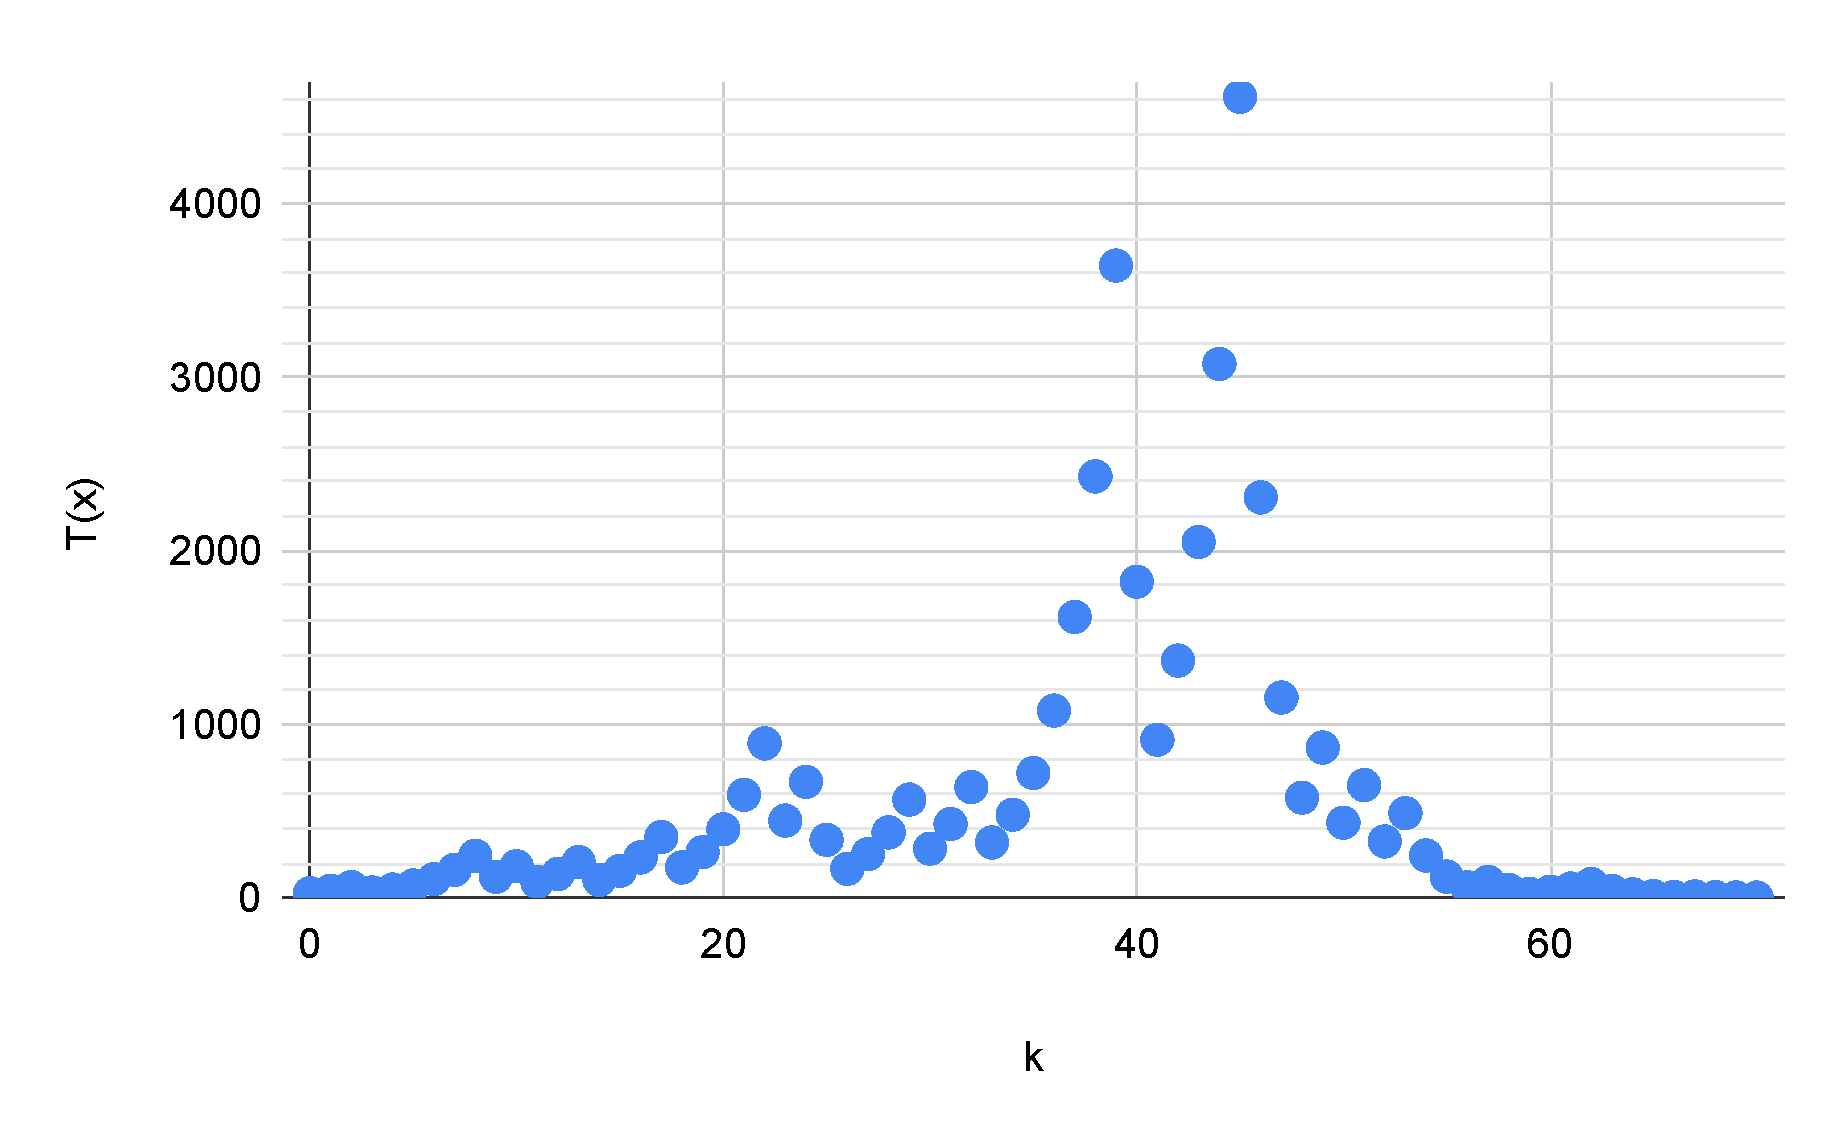
\includegraphics[width=\textwidth]{trajectory_27}
    \caption{The trajectory of $T^{(k)}(27)$ by number of iterations $k$}
\label{fig:01}
\end{figure}
One useful application of these stochastic approximations is the approximation
of the total stopping time of $T(x)$. This total stopping time is approximated 
to be $6.95212 \log x$ steps \cite{src:lagarias}.

\section{Examples}

This section demonstrates the trajectories, graphs, stopping times, and 
approximations to stopping times for the $3x+1$ functions of 27, 39, and 489. 
The computations for these examples were performed using a program written by 
the author in the C programming language and the graphs were created in Google 
Sheets using the resulting data.

\subsection{$T(x)$ for $x=27$}

The function $T(27)$ has a trajectory of length 70, so it is omitted here to 
save space. The graph of this trajectory is presented in \textsc{Figure} 
\ref{fig:01}. This graph shows how $T(x)$ changes pseudo-randomly when it is
iterated and shows that the function first climbs to a value of 4616 before it 
iterates to 1. \\
The stopping time is $\sigma(27)=59$, meaning it takes 59 iterations of $T(x)$
before the result is less than 27, in this case it is 23 at that point. The 
total stopping time is $\sigma_{\infty}(27)=70$. From this one knows that it 
takes 70 iterations of $T(x)$ to reach 1. Considering the stochastic 
approximation for the total stopping time ($6.95212 \log x$) one estimates that 
for $x=27$, $6.95212 \log 27 \approx 22.9131$ is the total stopping time. 
Considering that the true stopping time is 70, this is not a very good 
approximation. It has to be considered that the stopping time for 27 is 
unusually large for a number this small. But this shows that the approximation 
is, after all, just an approximation that has a certain accuracy.

\subsection{$T(x)$ for $x=39$}

The trajectory of $T(39)$ is 
\begin{align}
    \nonumber
    O^+(39):=\{&39,59,89,134,67,101,152,76,38,19,29,\\
    \nonumber
               &44,22,11,17,26,13,20,10,5,8,4,2,1\}.
\end{align}
The graph of this trajectory is presented in \textsc{Figure} \ref{fig:02}. 
Here, the highest value of the iteration is 152. The stopping time is 
$\sigma(39)=8$, meaning it takes 8 iterations of $T(x)$ for the result to be 
less than 39, in this case it is 38.
\begin{figure}[h]
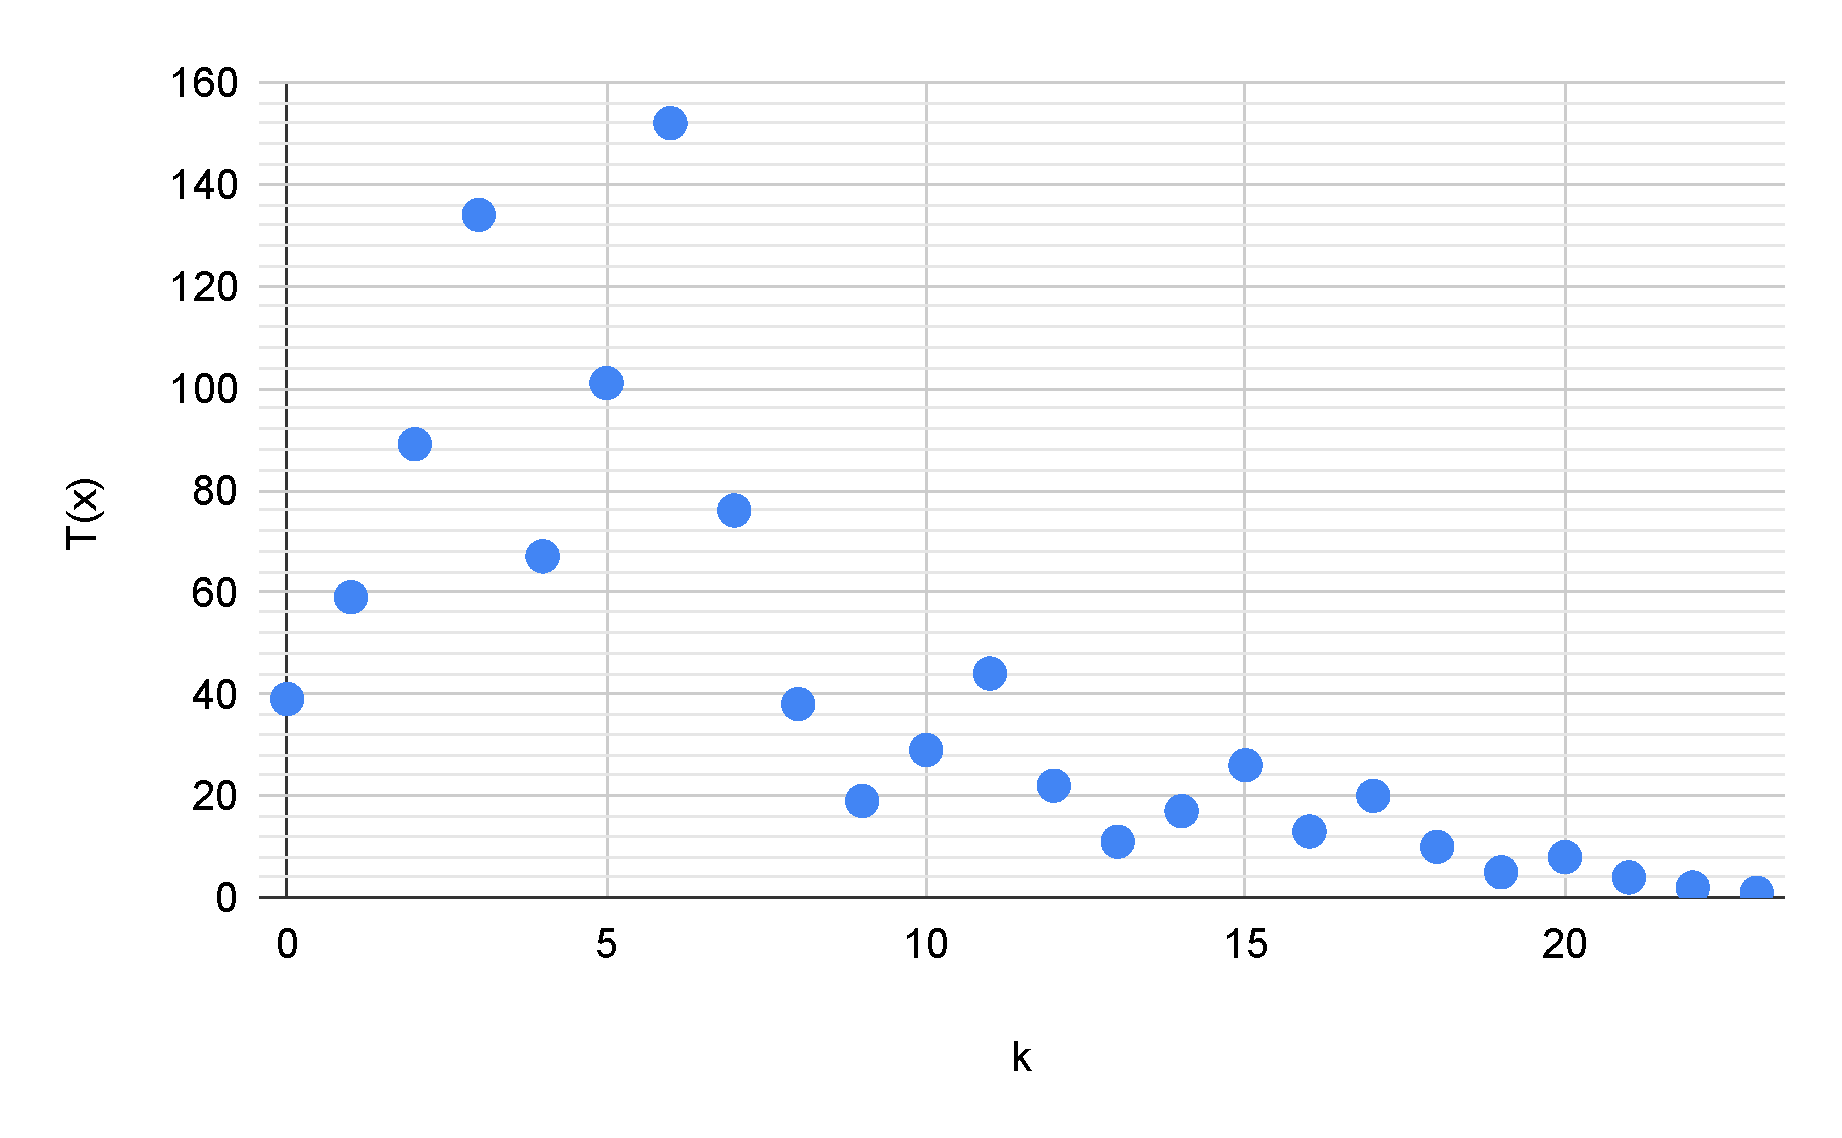
\includegraphics[width=\textwidth]{trajectory_39}
    \caption{The trajectory of $T^{(k)}(39)$ by number of iterations $k$}
\label{fig:02}
\end{figure}
The total stopping time is $\sigma_{\infty}(39)=23$. Thus, after 23 iterations 
of $T(x)$ the value of the function is 1. The stochastic approximation for the 
total stopping time for $T(39)$ is $6.95212 \log 39 \approx 25.46952$ compared
to the actual total stopping time 23. This approximation is better than the 
previous one for 27. This illustrates that these stochastic approximations vary 
in their accuracy for specific numbers because they are derived for groups of 
trajectories and large numbers and not single trajectories and small numbers.

\subsection{$T(x)$ for $x=489$}

For $T(489)$ the trajectory is 
\begin{align}
    \nonumber
    O^+(39):=\{&489,734,367,551,827,1241,1862,931,\\ \nonumber
               &1397,2096,1048,524,262,131,197,296,\\ \nonumber
               &148,74,37,56,28,14,7,11,17,26,13,20,\\ \nonumber
               &10, 5, 8, 4, 2, 1\}.
\end{align}
\begin{figure}[h]
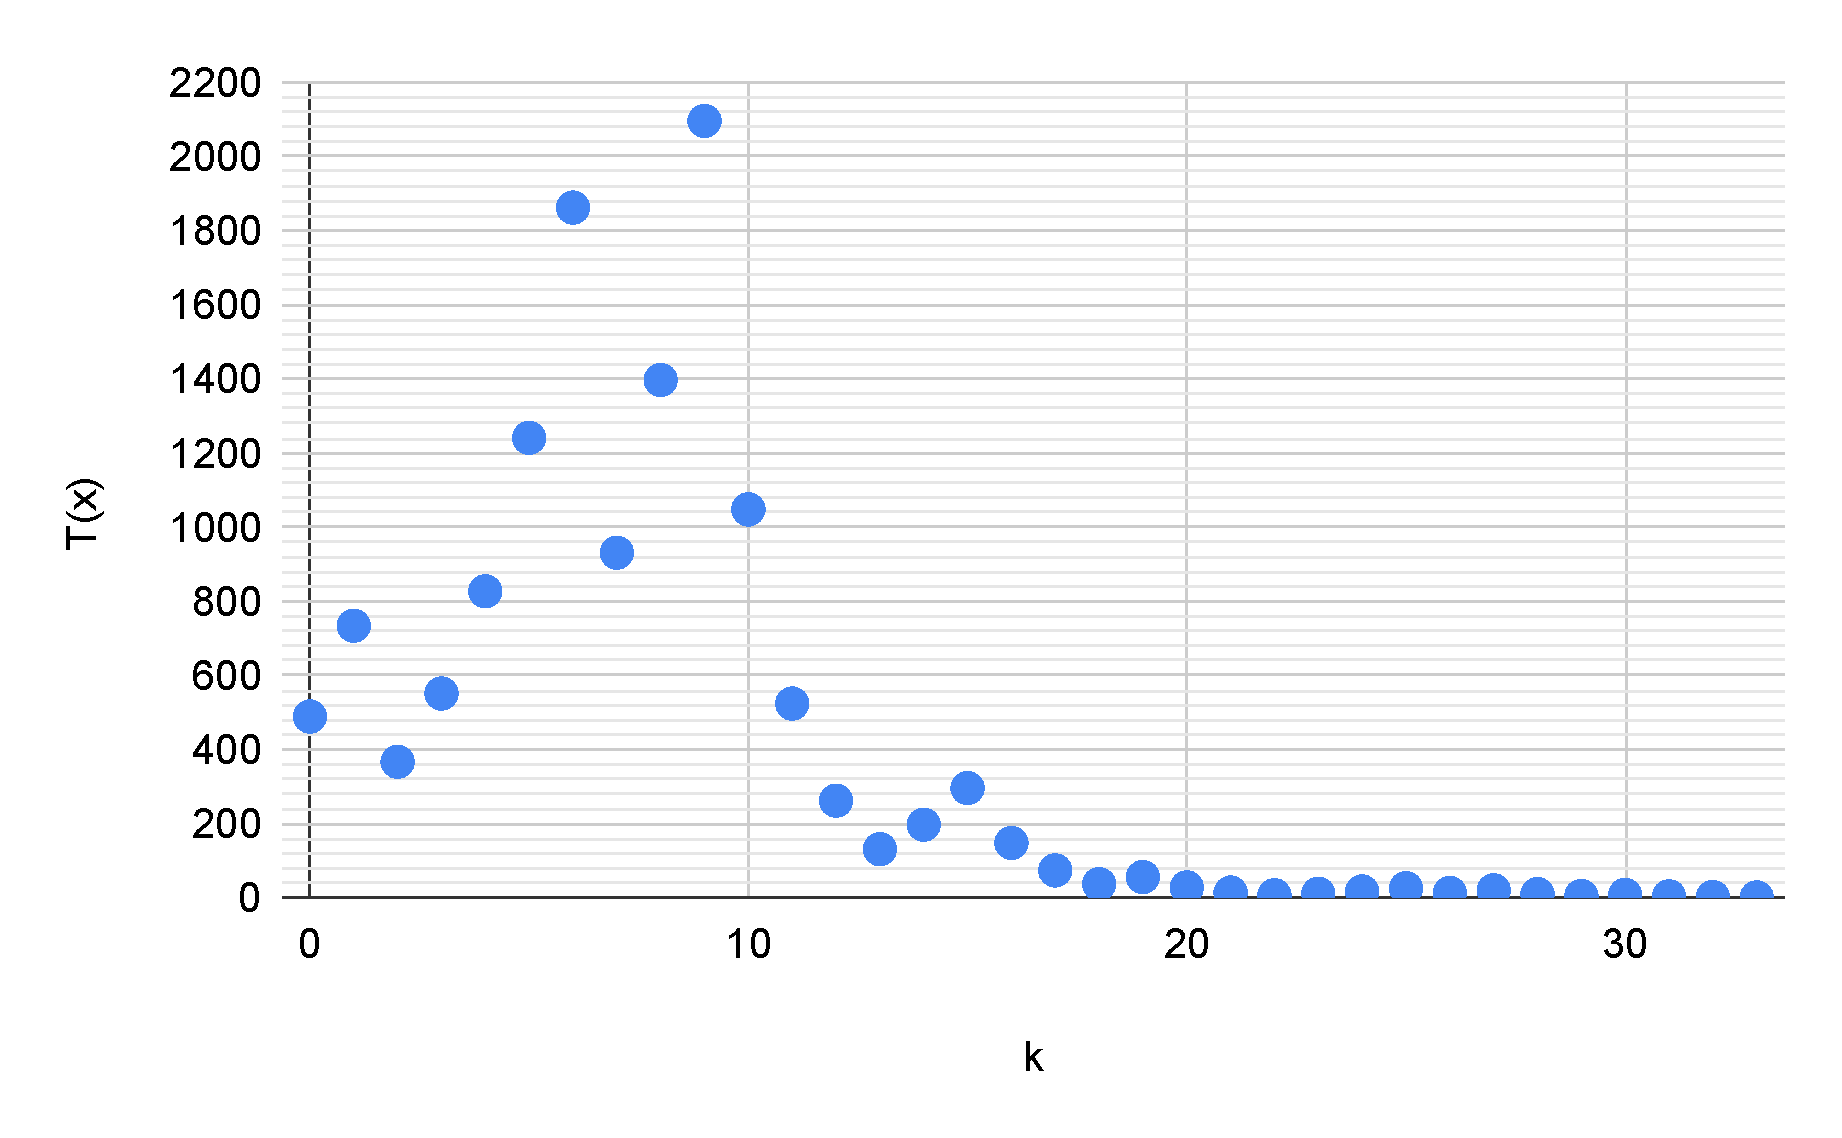
\includegraphics[width=\textwidth]{trajectory_489}
    \caption{The trajectory of $T^{(k)}(489)$ by number of iterations $k$}
\label{fig:03}
\end{figure}
\textsc{Figure} \ref{fig:03} shows the graph for this trajectory. The stopping
time in this case is $\sigma(489)=2$ because 367, which is smaller than 489, is
the second iteration of $T(x)$. The total stopping time of this iteration is 
$\sigma_{\infty}(489)=33$. In this case, estimating the total stopping time as 
$6.95212 \log 489 \approx 43.05$ compared to the real total stopping time 33 is 
relatively inaccurate compared to the previous one of $T(39)$. That is to be 
expected for an approximation that was, as previously mentioned, derived for 
large numbers. For example, for $x=2,234,567,899$, $\sigma_{\infty}(x)=147$ and 
$6.95212 \log (2,234,567,899) \approx 149.66$, which is a good estimate that
demonstrates that for larger numbers this estimation becomes more accurate.

\section{Conclusion}

The Collatz conjecture and the $3x+1$ problem are part of the field of number 
theory that is concerned with integer-valued functions. Research into the 
$3x+1$ problem is based on the $3x+1$ function $T(x)$ that maps positive 
integers to positive integers. The Collatz conjecture states that for every 
$x \in \mathbb{N} + 1$ there is a $k \in \mathbb{N} + 1$ such that 
$T^{(k)}(x)=1$. In over 50 years this conjecture has not been proven
\cite{src:lagarias}. \\
Using the help of computers, researchers have verified that the conjecture
holds for positive integers up to $10^{20}$ \cite{src:tao}. Concerning proofs, 
Terence Tao proved in \cite{src:tao} that almost all trajectories almost always 
go to 1. This represents progress towards proving the Collatz conjecture and 
shows that this problem is still being actively researched. \\
One of the challenging aspects of the $3x+1$ problem is its pseudo-random
nature. This arises because $T(x)$ behaves in a hard-to-predict manner when it
is iterated. Because mathematical proofs generally rely on patterns and
regularity, this randomness makes the proof even more difficult. An unexpected
implication of this pseudo-randomness is the fact that is allows mathematicians
to describe groups of trajectories using probabilistic functions and to make
approximations about its behavior. For example, this allows the number of
iterations $k$ of $T(x)$ to be estimated \cite{src:lagarias}. \\
To conclude, the $3x+1$ problem is an interesting problem in number theory that
is easy to state and understand but extremely difficult to prove. If it were to
get proven the results could have implications for other areas of mathematics
and computer science.

\begin{thebibliography}{4}

\bibitem{src:chamberland} Marc Chamberland, 
    \textit{An Update on the $3x+1$ Problem}, 
    \texttt{http://www.math.grinnell.edu/\\
        \~{}chamberl/papers/3x\_survey\_eng.pdf}, 2005.

\bibitem{src:lagarias} Jeffrey C. Lagarias, 
    \textit{The $3x+1$ Problem: An Overview}, 
    \texttt{https://pdfs.semanticscholar.\\
        org/100046dd8b4ee901bc71043da7d42f5d87ca0224.pdf}, 2010.

\bibitem{src:tao} Terence Tao, \textit{Almost All Orbits of the Collatz Map Attain
    Almost Bounded Values}, arXiv:1909.03562v2 [math.PR], 2019.

\end{thebibliography}

\end{document}
